%%%%%%%%%%%%%%%%%%%%%%%%%%%%%%%%%%%%%%%
%%% COLISOES
%   Aplicacao das colisoes e criterios. Exemplos do uso
%   para problemas de poucos corpos e problemas de varios
%   corpos. Custo computacional e eficiencia.
%%%%%%%%%%%%%%%%%%%%%%%%%%%%%%%%%%%%%%%
\section{Colisões}\label{section:simulacao_colisoes}
Como inicialmente discutido na seção \ref{section:pncg_colisoes}, existem algumas formas de lidar com colisões no PNCG e que se aplicam para aproximações muito intensas, ou \textit{quase colisões}, uma vez que o conjunto de valores iniciais que levam a uma colisão em tempo finito têm medida zero. A abordagem com colisões elásticas é uma delas.

Para utilizar colisões, como já dito, um meio natural é definir uma densidade $\rho$ para a massa de modo que
\begin{equation}
    r_a = \sqrt[3]{\dfrac{3 m_a}{4 \pi \rho}}
\end{equation}
é o raio de um corpo esférico de massa $m_a$. Cada escolha de densidade possível gera um conjunto de trajetórias diferentes, uma vez que uma aproximação intensa que é considerada como colisão para um certo $\rho_1$ pode não o ser para um $\rho_2$ diferente. Porém, este método possui a vantagem de garantir a reprodutibilidade das simulações.

Um problema de utilizar colisões elásticas é que nem sempre o raio é o suficiente para detectar uma colisão ou quase-colisão antes que o estrago numérico seja feito. Pode acontecer, por exemplo, de em um instante $t$ dois corpos estarem distantes o suficiente para não haver colisão mas no instante $t + \delta t$ os dois volumes associados aos corpos terem uma interseção não vazia no espaço de configurações - na prática, um corpo \textit{entrar} no outro, como na figura \ref{fig:colisao_intersecao}. Uma tática que pode ser utilizada para evitar isso é: uma vez detectada a interseção, interpolar as trajetórias entre os instantes $t$ e $t+\delta t$, obtendo assim o exato momento da colisão $t \leq t^* \leq t+\delta t$, aplicar a colisão em $t^*$ e substituir a trajetória com interseção em $t + \delta t$ pela trajetória em que houve colisão no instante $t^*$. Embora não exista dificuldade teórica em tal tática, aplicá-la numericamente é um desafio, especialmente em problemas de muitos corpos, pois todo esse processo é, além de custoso, computacionalmente complicado de ser avaliado, por isso não foi utilizado.

\begin{figure}
    \centering
    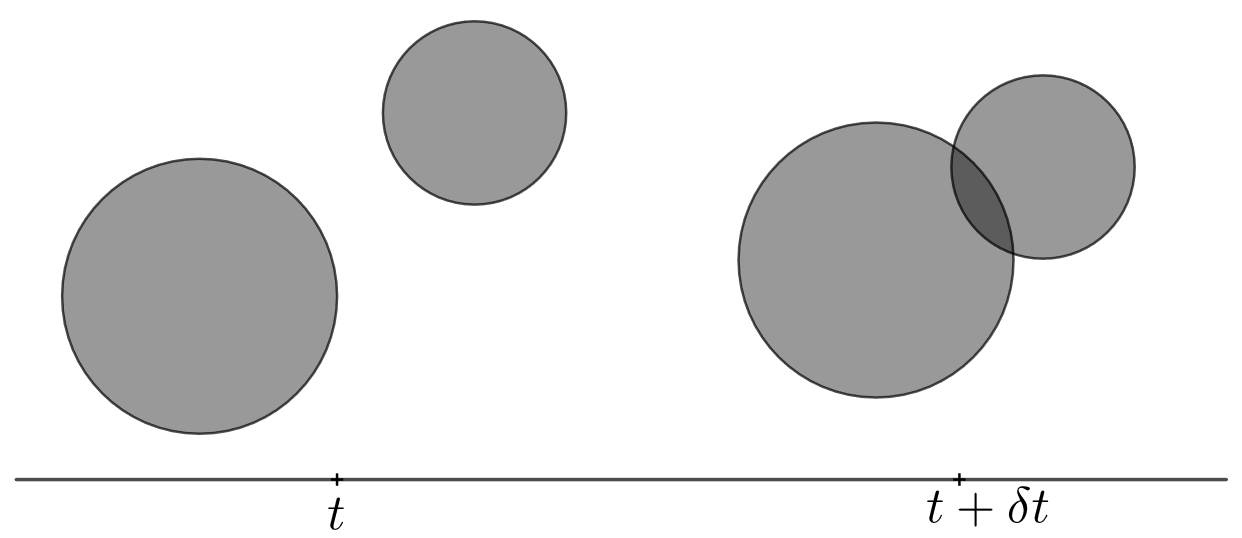
\includegraphics[width=0.7\linewidth]{tcc//img/colisao_intersecao.png}
    \caption{Problema descrito, onde o instante de colisão exato $t^*$ é tal que $t \leq t^* \leq t + \delta t$}
    \label{fig:colisao_intersecao}
\end{figure}

Outra saída mais simples para o problema é: uma vez detectada uma aproximação no instante $t+\delta t$ intensa o suficiente para desestabilizar numericamente o sistema antes de uma colisão elástica surtir efeito, voltar para o instante $t$ e aplicar a colisão elástica neste instante. Existem dois problemas com essa tática: é preciso escolher mais um valor $\epsilon_E$ (ligado à energia) para poder definir o que é uma \textit{desestabilização} considerável e é possível que retornar ao passo anterior resolva o problema de imediato, mas jogue a partícula colidida em rota de colisão com outra partícula, gerando uma situação recursiva.

O primeiro problema poderia ser resolvido com estatística, identificando uma ``desestabilização'' como um \textit{outlier} numa estatística suficiente para a energia, por exemplo, ou com o rigor dos integradores numéricos, pois cada integrador tem um teto para o erro das trajetórias e consequentemente um teto para o erro da energia total, sendo uma ``desestabilização'' qualquer coisa acima dessa margem. A solução estatística chegou a ser brevemente testada mas não ofereceu resultados satisfatórios, uma vez que trouxe mais um custo computacional e não foi capaz de se livrar do segundo problema. A solução com teto dos integradores não foi implementada por dificuldades teóricas em determinar o teto, mas pretendemos avaliar essa medida de erro de cada método no futuro.

Uma última questão com as colisões elásticas é o custo de identificar seu acontecimento. Da mesma forma que o potencial e as forças, são necessárias $N (N-1) / 2$ verificações para identificar uma colisão, sendo então mais uma operação computacionalmente custosa. Existem outras formas mais eficientes de detectar colisões e há toda uma literatura voltada para isso, como \cite{Ericson2005}, pois existe uma gama de aplicações que necessitam de métodos eficientes para detecção de colisões. Para este trabalho, por facilidade, foi utilizada a verificação um-a-um comentada.

Existem outras regularizações que permitem lidar com colisões, especialmente colisões binárias, como a transformação de Levi-Civita (para problemas planares), sua generalização no método de Kustaanheimo-Stiefel e a alternativa pelo método de Burdet-Heggie \citep{aarseth_gravitational_2003}. Nenhuma dessas regularizações foi estudada a fundo então estas não serão tratadas neste trabalho. Para mais detalhes, a referência de Aarseth é recomendada para os três métodos mencionados, tendo o seu capítulo 4 totalmente voltado para este problema.

Há também outra forma de evitar colisões e quase-colisões, que é impondo um limite sobre o potencial. Tomando $\epsilon > 0$, definimos o potencial amortecido
\begin{equation}
    V_\epsilon = - G \sum_{a < b} \dfrac{m_a m_b}{\sqrt{r_{ab}^2 + \epsilon^2}},
\end{equation}
o que gera as forças
\begin{equation}
    \derpar{V}{\vet q_a} = G \sum_{b \neq a} m_a m_b \dfrac{\vet q_b - \vet q_a}{(r_{ab}^2 + \epsilon^2)^{3/2}}.
\end{equation}

Observe que apesar da diferença nos cálculos, a energia total amortecida $E_\epsilon = T + V_\epsilon$ ainda é conservada, pois
\begin{equation*}
    \der{E_\epsilon}{t} 
    = \nabla_{\vet p} T \cdot \dvet p + \nabla_{\vet q} V_\epsilon \cdot \dvet q
    = 0.
\end{equation*}

O uso de um amortecimento pode levantar dúvidas naturais a respeito da precisão dos resultados obtidos com simulações. É fato que o mesmo conjunto de valores iniciais leva a um resultado quando usado o potencial $V$ e a outro resultado quando usado o potencial $V_\epsilon$. Porém, quando o interesse está nas propriedades dinâmicas do sistema e não em trajetórias individuais - o que no geral ocorre para valores de $N$ suficientemente grandes -, $\epsilon$ precisa ser relativamente grande para que o resultado final seja notavelmente diferente \citep[235]{aarseth_gravitational_2003}.

Dessa forma, tanto a colisão elástica quanto o potencial amortecido conservam a energia de alguma forma, então foram implementados no programa final. Cabe observar que uma possível solução para se livrar de alguns dos problemas comentados no uso de colisões elásticas é utilizar um método híbrido que incorpore o amortecimento, além de utilizar o corretor para amenizar a instabilidade do potencial. Ainda assim, é esperado que as órbitas individuais sejam diferentes, mesmo que as integrais primeiras sejam as mesmas. Um exemplo pode ser visto na figura \ref{fig:iau25_trajetorias_colisoes}.

\begin{figure}
    \centering
    \begin{subfigure}{.5\textwidth}
      \centering
      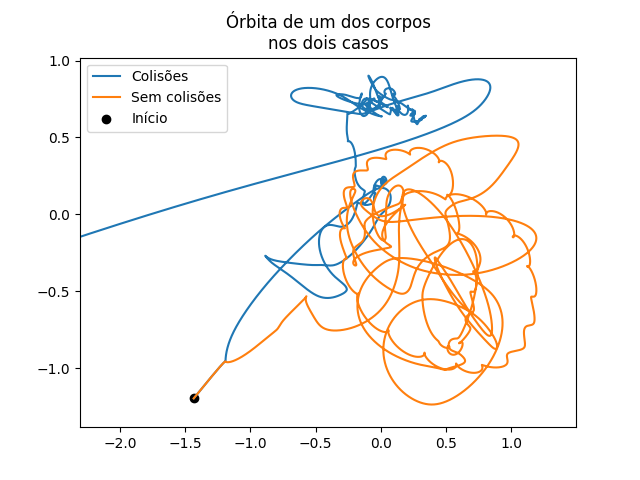
\includegraphics[width=\linewidth]{tcc/img/trajetoria_iau25_colisao_vs_sem_colisao.png}
      % \caption{Órbita de um dos corpos nos dois casos.}
      \caption{}
      \label{fig:iau25_trajetorias_colisoes_a}
    \end{subfigure}%
    \begin{subfigure}{.5\textwidth}
      \centering
      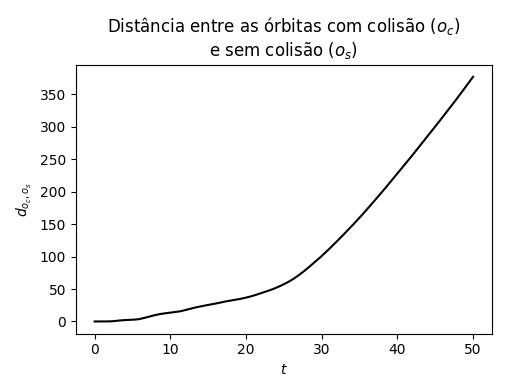
\includegraphics[width=\linewidth]{tcc/img/distancia_orbitas_iau25.png}
      % \caption{Distância entre as órbitas no espaço de fases.}
      \caption{}
      \label{fig:iau25_trajetorias_colisoes_b}
    \end{subfigure}
    
    \caption{Simulações do problema-modelo \ref{probmodelo:iau25} via método RKN671 com $h=10^{-3}$, $\epsilon=5h$ e corretor com margem de erro da energia $10^{-10}$ no intervalo $[0,50]$. Em um dos casos utilizou-se colisões ativadas com $r_a = 5h$, $a=1,2,...,N$ e no outro as colisões estavam desativadas.}
    \label{fig:iau25_trajetorias_colisoes}
\end{figure}